\ifx\pdfminorversion\undefined\else\pdfminorversion=4\fi
\documentclass[aspectratio=169,t]{beamer}
%\documentclass[aspectratio=169,t,handout]{beamer}

% English version FAU Logo
\usepackage[english]{babel}
% German version FAU Logo
%\usepackage[ngerman]{babel}

\usepackage[utf8]{inputenc}
\usepackage[T1]{fontenc}
\usepackage{amsmath,amssymb}
\usepackage{graphicx}
\usepackage{listings}
\usepackage{url}
\usepackage{enumitem}
\usepackage{hyperref}
\usepackage{fontawesome}
\usepackage{graphicx}
\usepackage{booktabs}
\usepackage{calc}
\usepackage{ifthen}
\usepackage{xcolor}
\usepackage{tabularx}
\usepackage{tikz}
\usepackage{tikz}
\usepackage{tikz-cd}
\usepackage{verbatim}
\usepackage{pgfplots,pgfplotstable,pgf-pie}
\usepackage{filecontents}
\newcommand{\plots}{0.611201}
\newcommand{\plotm}{2.19882}
\pgfplotsset{height=4cm,width=8cm,compat=1.17}
\pgfmathdeclarefunction{gauss}{2}{%
  \pgfmathparse{1/(#2*sqrt(2*pi))*exp(-((x-#1)^2)/(2*#2^2))}%
}

\tikzset{
    vertex/.style = {
        circle,
        fill            = black,
        outer sep = 2pt,
        inner sep = 1pt,
    }
}

\tikzset{
    mynode/.style={
        draw,
        thick,
        anchor=south west,
        minimum width=2cm,
        minimum height=1.3cm,
        align=center, 
        inner sep=0.2cm,
        outer sep=0,
        rectangle split, 
        rectangle split parts=2,
        rectangle split draw splits=false},
    reverseclip/.style={
        insert path={(current page.north east) --
            (current page.south east) --
            (current page.south west) --
            (current page.north west) --
            (current page.north east)}
    }
}

\tikzset{basic/.style={
        draw,
        rectangle split,
        rectangle split parts=2,
        rectangle split part fill={blue!20,white},
        minimum width=2.5cm,
        text width=2cm,
        align=left,
        font=\itshape
    },
    Diamond/.style={ diamond, 
                      draw, 
                      shape aspect=2, 
                      inner sep = 2pt,
                      text centered,
                      fill=blue!10!white,
                      font=\itshape
                    }}


\tikzset{level 1/.append style={sibling angle=50,level distance = 165mm}}
\tikzset{level 2/.append style={sibling angle=20,level distance = 45mm}}
\tikzset{every node/.append style={scale=1}}

\usetikzlibrary{arrows,decorations.pathmorphing,backgrounds,fit,positioning,shapes.symbols,chains,intersections,snakes,positioning,matrix,mindmap,shapes.multipart,shapes,calc,shapes.geometric}

% read in data file


\newcommand{\MaxNumberX}{3}
\newcommand{\MaxNumberY}{5}
\newcommand{\tikzmark}[1]{\tikz[remember picture] \node[coordinate] (#1) {#1};}

\pgfplotstableread{data/iris.dat}\iris
\pgfplotstablegetrowsof{\iris}
\pgfplotsset{compat=1.14}
\pgfmathsetmacro\NumRows{\pgfplotsretval-1}
\definecolor{airforceblue}{rgb}{0.36, 0.54, 0.66}

\usepgfplotslibrary{groupplots}
% Options:
%  - inst:      Institute
%                 med:      MedFak FAU theme
%                 nat:      NatFak FAU theme
%                 phil:     PhilFak FAU theme
%                 rw:       RWFak FAU theme
%                 rw-jura:  RWFak FB Jura FAU theme
%                 rw-wiso:  RWFak FB WISO FAU theme
%                 tf:       TechFak FAU theme
%  - image:     Cover image on title page
%  - plain:     Plain title page
%  - longtitle: Title page layout for long title
\usetheme[%
  image,%
  longtitle,%
  tf
]{fau}

% Enable semi-transparent animation preview
\setbeamercovered{transparent}


\lstset{%
  language=Python,
  tabsize=2,
  basicstyle=\tt,
  keywordstyle=\color{blue},
  commentstyle=\color{green!50!black},
  stringstyle=\color{red},
  numbers=left,
  numbersep=0.5em,
  xleftmargin=1em,
  numberstyle=\tt
}


% Title, authors, and date
\title[KDD]{Chapter V: Mining frequent patterns, associations and correlations}
\subtitle{Knowledge Discovery in Databases}
\author[L.~Melodia]{Luciano Melodia M.A.}
% English version
\institute[Department]{Evolutionary Data Management, Friedrich-Alexander University Erlangen-Nürnberg}
% German version
%\institute[Lehrstuhl]{Lehrstuhl, Friedrich-Alexander-Universit\"at Erlangen-N\"urnberg}
\date{Summer semester 2021}
% Set additional logo (overwrites FAU seal)
%\logo{\includegraphics[width=.15\textwidth]{themefau/art/xxx/xxx.pdf}}
\begin{document}
  % Title
  \maketitle

  { 
    \setbeamertemplate{footline}{}
    \begin{frame}{Chapter V: Mining frequent patterns, associations and correlations}
        \begin{itemize}
            \item \textbf{Basic Concepts.}
            \item Scalable frequent-itemset-mining methods.
            \begin{itemize}
              \item Apriori: a candidate-generation-and-test approach.
              \item Improving the efficiency of apriori.
              \item FPGrowth:  a frequent-pattern-growth approach.
              \item ECLAT: frequent-pattern mining with vertical data format.
              \item Mining closed itemsets and max-itemsets.
            \end{itemize}
            \item Generating association rules from frequent itemsets.
            \item Which patterns are interesting? Pattern-evaluation methods.
            \item Summary.
        \end{itemize}
    \end{frame}
  }

  { 
    \setbeamertemplate{footline}{}
    \begin{frame}{What is frequent-pattern analysis?}
        \begin{itemize}
            \item \textbf{Frequent pattern:}
            \begin{itemize}
              \item A pattern (a set of items, subsequences, substructures, etc.) that occurs frequently in a dataset.
              \item A pattern (a set of items, subsequences, substructures, etc.) that occurs frequently in a dataset.
            \end{itemize}
            \item \textbf{Motivation: Finding inherent regularities in data:}
            \begin{itemize}
              \item What products are often purchased together? Beer and diapers?!
              \item What are the subsequent purchases after buying a PC?
              \item FPGrowth: a frequent-pattern-growth approach.
              \begin{itemize}
                \item "Who bought this has often also bought $\ldots$"
              \end{itemize}
              \item What kinds of DNA are sensitive to this new drug?
              \item Can we automatically classify Web documents?
            \end{itemize}
            \item \textbf{Applications:}
            \begin{itemize}
              \item Basket-data analysis, cross-marketing, catalog design, sale-campaign analysis, Web-log (click-stream) analysis, and DNA-sequence analysis.
            \end{itemize}
        \end{itemize}
    \end{frame}
  }

  { 
    \setbeamertemplate{footline}{}
    \begin{frame}{Why is frequent-pattern mining important?}
        \begin{itemize}
            \item \textbf{A frequent pattern is an intrinsic and important property of a dataset.}
            \item \textbf{Foundation for many essential data-mining tasks:}
            \begin{itemize}
              \item Association, correlation, and causality analysis.
              \item Sequential, structural (e.g., sub-graph) patterns.
              \item Pattern analysis in spatiotemporal, multimedia, time-series, and stream data.
              \item Classification: discriminative, frequent-pattern analysis.
              \item Cluster analysis: frequent-pattern-based clustering.
              \item Data warehousing: iceberg cube and cube gradient.
              \item Semantic data compression: fascicles (Jagadish, Madar, and Ng, VLDB'99).
              \item Broad applications.
            \end{itemize}
        \end{itemize}
    \end{frame}
  }


  { 
    \setbeamertemplate{footline}{}
    \begin{frame}{An example}
        \begin{itemize}
            \item \textbf{From: Martin Lindstrom: Brandwashed. Random House, 2011:}
            \item \begin{quote}
            It is by crunching these numbers that the data-mining industry has uncovered some even more surprising factoids:

            Did you know, for example, that at Walmart a shopper who buys a Barbie doll is 60 percent more likely to purchase one of three types of candy bars? Or that toothpaste is most often bought alongside canned tuna? Or that a customer who buys a lot of meat is likely to spend more money in a health-food store than a non-meat-eater? Or what about the data revealed to one Canadian grocery chain that customers who bought coconuts also tended to buy prepaid calling cards? At first, no one in store management could figure out what was going on. What could coconuts possibly have to do with calling cards?

            Finally it occurred to them that the store served a huge population of shoppers from the Caribbean islands and Asia, both of whose cuisines use coconuts in their cooking. Now it made perfect sense that these Caribbean and Asian shoppers were buying prepaid calling cards to check in with their extended families back home.
            \end{quote}
        \end{itemize}
    \end{frame}
  }

  { 
    \setbeamertemplate{footline}{}
    \begin{frame}{An example}
        \begin{columns}
          \begin{column}{0.4\textwidth}
          \begin{tabular}{|c|c|}
          \hline
          \textbf{TID} & \textbf{Items bought}\\\hline
          10 & Beer, Nuts, Diapers \\\hline
          20 & Beer, Coffee, Diapers \\\hline
          30 & Beer, Diapers, Eggs \\\hline
          40 & Nuts, Eggs, Milk \\\hline
          50 & Nuts, Coffee, Diapers, Eggs, Milk\\\hline
          \end{tabular}
          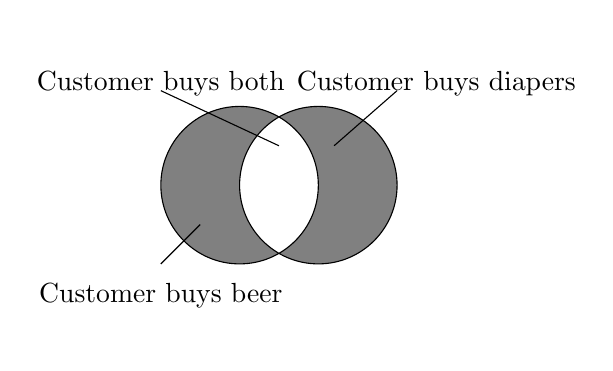
\begin{tikzpicture}[fill=gray]
          % left hand
          \scope
          \clip (-2,-2) rectangle (2,2)
                (1,0) circle (1);
          \fill (0,0) circle (1);
          \endscope
          % right hand
          \scope
          \clip (-2,-2) rectangle (2,2)
                (0,0) circle (1);
          \fill (1,0) circle (1);
          \endscope
          % outline
          \draw (0,0) circle (1) (0,1) (1,0) circle (1) (1,1);
          \node[label=below:{Customer buys beer}] at (-1,-1) {};
          \node[label=below:{Customer buys diapers}] at (2.5,1.7) {};
          \node[label=below:{Customer buys both}] at (-1,1.7) {};
          \draw (-1,-1) -- (-0.5,-0.5);
          \draw (2,1.2) -- (1.2,0.5);
          \draw (-1,1.2) -- (0.5,0.5);
          \end{tikzpicture}
          \end{column}
          \begin{column}{0.5\textwidth}
          \vspace{-2cm}
          \begin{itemize}
            \item \textbf{Itemset:}
            \begin{itemize}
              \item A set of one or more items.
              \item $k$-itemset $X = \{x_1, x_2, \ldots, x_k\}$.
            \end{itemize}
            \item \textbf{(Absolute) Support, or support count of $X$:}
            \begin{itemize}
              \item Frequency or occurrence of $X$.
            \end{itemize}
            \item (Relative) Support $s$:
            \begin{itemize}
              \item The fraction of the transactions that contain $X$.
              \item I.e. the \textbf{probability} that a transaction contains $X$.
            \end{itemize}
            \item \textbf{An itemset $X$ is frequent, if $X$'s support is no less than a \texttt{min\_sup} threshold.}
          \end{itemize}
          \end{column}
        \end{columns}
    \end{frame}
  }

  { 
    \setbeamertemplate{footline}{}
    \begin{frame}{An example}
        \begin{columns}
          \begin{column}{0.4\textwidth}
          \begin{tabular}{|c|c|}
          \hline
          \textbf{TID} & \textbf{Items bought}\\\hline
          10 & Beer, Nuts, Diapers \\\hline
          20 & Beer, Coffee, Diapers \\\hline
          30 & Beer, Diapers, Eggs \\\hline
          40 & Nuts, Eggs, Milk \\\hline
          50 & Nuts, Coffee, Diapers, Eggs, Milk\\\hline
          \end{tabular}
          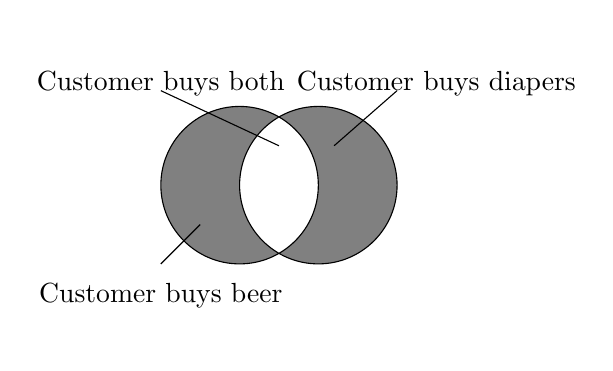
\begin{tikzpicture}[fill=gray]
          % left hand
          \scope
          \clip (-2,-2) rectangle (2,2)
                (1,0) circle (1);
          \fill (0,0) circle (1);
          \endscope
          % right hand
          \scope
          \clip (-2,-2) rectangle (2,2)
                (0,0) circle (1);
          \fill (1,0) circle (1);
          \endscope
          % outline
          \draw (0,0) circle (1) (0,1) (1,0) circle (1) (1,1);
          \node[label=below:{Customer buys beer}] at (-1,-1) {};
          \node[label=below:{Customer buys diapers}] at (2.5,1.7) {};
          \node[label=below:{Customer buys both}] at (-1,1.7) {};
          \draw (-1,-1) -- (-0.5,-0.5);
          \draw (2,1.2) -- (1.2,0.5);
          \draw (-1,1.2) -- (0.5,0.5);
          \end{tikzpicture}
          \end{column}
          \begin{column}{0.5\textwidth}
          \vspace{-2cm}
          \begin{itemize}
            \item \textbf{Find all the rules $X \rightarrow Y$ with minimum support and confidence.}
            \begin{itemize}
              \item \textbf{Support} $s$: probability that a transaction contains $X \cup Y$.
              \item \textbf{Confidence} $c$: conditional probability that a transaction having $X$ also contains $Y$.
            \end{itemize}
            \item \textbf{Example:}
            \begin{itemize}
              \item Let $\text{min\_sup} = 50\%$ and $\text{min\_conf} = 50\%$.
              \item Frequent itemsets:
              \begin{itemize}
                \item Beer: $3$, Nuts: $3$,
                \item Diapers: $4$, Eggs: $3$,
                \item $\{\text{Beer, Diapers}\}$: $3$.
              \end{itemize}
              \item \textbf{Association rules:}
              \begin{itemize}
                \item Beer $\rightarrow$ Diapers ($60\%$, $100\%$).
                \item Diapers $\rightarrow$ Beer ($60\%$, $75\%$).
              \end{itemize}
            \end{itemize}
          \end{itemize}
          \end{column}
        \end{columns}
    \end{frame}
  }

  { 
    \setbeamertemplate{footline}{}
    \begin{frame}{Basic concepts: association rules (2)}
    \begin{itemize}
      \item \textbf{Implikation of the form $A \rightarrow B$:}
      \begin{itemize}
        \item where $A \neq \emptyset$, $B \neq \emptyset$ and $A \cap B = \emptyset$.
      \end{itemize}
      \item \textbf{Strong rule:}
      \begin{itemize}
        \item Satisfies both $\text{min\_sup}$ and $\text{min\_conf}$
        \begin{align}
        \text{support}(A \rightarrow B) &= P(A \cup B),\\
        \text{confidence}(A \rightarrow B) &= P(B | A)\\
        &= \frac{\text{support}(A \cup B)}{\text{support}(A)}\\
        &= \frac{\text{support\_count}(A\cup B)}{\text{support\_count}(A)}.
        \end{align}
        \item I.e. confidence of rule can be easily derived from the support counts of $A$ and $A \cup B$.
      \end{itemize}
      \item \textbf{Association-rule mining:}
      \begin{itemize}
        \item Find all frequent itemsets.
        \item Generate strong association rules from the frequent itemsets.
      \end{itemize}
    \end{itemize}
    \end{frame}
  }

  { 
    \setbeamertemplate{footline}{}
    \begin{frame}{Closed itemsets and max-itemsets}
    \begin{itemize}
      \item \textbf{A long itemset contains a combinatorial number of sub-itemsets.}
      \begin{itemize}
        \item E.g. $\{a_1,a_2,\ldots,a_{100}\}$ contains
        \begin{align}
        {100\choose 1} + {100 \choose 2} + \cdots + {100 \choose 100} = 2^{100}-1 \approx 1.27 \cdot 10^{30} \; \text{sub-itemsets!}
        \end{align}
        \item \textbf{Solution:}
        \begin{itemize}
          \item Mine closed itemsets and max-itemsets instead.
        \end{itemize}
        \item \textbf{An itemset $X$ is closed, if $X$ is frequent and there exists no super-itemset $X \subset Y$ with the same support as $X$.}
        \begin{itemize}
          \item Proposed by (Pasquier et al., ICDT'99).
        \end{itemize}
        \item \textbf{An itemset $X$ is a max-itemset, if $X$ is frequent and there exists no frequent super-itemset $X \subset Y$.}
        \begin{itemize}
          \item Proposed by (Bayardo, SIGMOD'98).
        \end{itemize}
        \item \textbf{Closed itemset is a lossless "compression" of frequent itemsets.}
        \begin{itemize}
          \item Reducing the number of itemsets (and rules).
        \end{itemize}
      \end{itemize}
    \end{itemize}
    \end{frame}
  }

  { 
    \setbeamertemplate{footline}{}
    \begin{frame}{Closed itemsets and max-itemsets (II)}
    \begin{itemize}
      \item \textbf{Example:}
      \begin{itemize}
        \item $\text{DB} = \{\langle a_1,a_2, \ldots, a_{100} \rangle, \langle a_1, a_2, \ldots, a_{100} \rangle \}$.
        \item I.e. just two transactions.
        \item $\text{min\_sup} = 1$.
      \end{itemize}
      \item \textbf{What are the closed itemsets?}
      \begin{itemize}
        \item $\langle a_1,a_2, \ldots, a_{100} \rangle : 1$,
        \item $\langle a_1,a_2, \ldots, a_{50} \rangle : 2$,
        \item Number behind the colon: support\_count.
      \end{itemize}
      \item \textbf{What are the max-itemsets?}
      \begin{itemize}
        \item $\langle a_1,a_2, \ldots, a_{100} \rangle : 1$.
      \end{itemize}
      \item \textbf{What is the set of all frequent itemsets?}
    \end{itemize}
    \end{frame}
  }

  { 
    \setbeamertemplate{footline}{}
    \begin{frame}{Chapter V: Mining frequent patterns, associations and correlations}
        \begin{itemize}
            \item Basic Concepts.
            \item \textbf{Scalable frequent-itemset-mining methods.}
            \begin{itemize}
              \item \textbf{Apriori: a candidate-generation-and-test approach.}
              \item Improving the efficiency of apriori.
              \item FPGrowth:  a frequent-pattern-growth approach.
              \item ECLAT: frequent-pattern mining with vertical data format.
              \item Mining closed itemsets and max-itemsets.
            \end{itemize}
            \item Generating association rules from frequent itemsets.
            \item Which patterns are interesting? Pattern-evaluation methods.
            \item Summary.
        \end{itemize}
    \end{frame}
  }

  {
    \setbeamertemplate{footline}{}
    \begin{frame}{The downward-closure property and scalable mining methods}
    \begin{itemize}
      \item \textbf{The downward-closure property of frequent patterns:}
      \begin{itemize}
        \item \textbf{\color{airforceblue}Any subset of a frequent itemset must also be frequent.}
        \begin{itemize}
          \item If $\{\text{Beer, Diapers, Nuts}\}$ is frequent, so is $\{\text{Beer, Diapers}\}$.
          \item I.e. every transaction having $\{\text{Beer, Diapers, Nuts}\}$ also contains $\{\text{Beer, Diapers}\}$.
        \end{itemize}
      \end{itemize}
      \item \textbf{Scalable mining methods: three major approaches.}
      \begin{itemize}
        \item A priori (Agrawal \& Srikant, VLDB'94).
        \item Frequent-pattern growth (FPgrowth) (Han, Pei \& Yin, SIGMOD'00).
        \item Vertical-data-format approach (CHARM) (Zaki \& Hsiao, SDM'02).
      \end{itemize}
    \end{itemize}
    \end{frame}
  }

  {
    \setbeamertemplate{footline}{}
    \begin{frame}{A priori: a candidate generation \& test approach}
    \begin{itemize}
      \item \textbf{A priori pruning principle:}
      \begin{itemize}
        \item \textbf{\color{airforceblue}If there is any itemset which is infrequent, \\ its supersets should not be generated/tested!} \\ (Agrawal \& Srikant, VLDB'94; Mannila et al., KDD'94)
      \end{itemize}
      \item \textbf{Method:}
      \begin{itemize}
        \item Initially, scan DB once to get frequent $1$-itemsets.
        \item Generate length-$(k+1)$ candidate itemsets from length-$k$ frequent itemsets.
        \item Test the candidates against DB, discard those that are infrequent.
        \item Terminate when no further candidate or frequent itemset can be generated.
      \end{itemize}
    \end{itemize}
    \end{frame}
  }


  {
    \setbeamertemplate{footline}{}
    \begin{frame}{References: Basic concepts of frequent-pattern mining}
    \begin{itemize}
      \item (Association Rules)
      \begin{itemize}
        \item R. Agrawal, T. Imielinski, and A. Swami: Mining association rules between sets of items in large databases. SIGMOD'93.
      \end{itemize}
      \item (Max-Itemset)
      \begin{itemize}
        \item (Max-Itemset) R. J. Bayardo: Efficiently mining long patterns from databases. SIGMOD'98.
      \end{itemize}
      \item (Closed Itemsets)
      \begin{itemize}
        \item N. Pasquier, Y. Bastide, R. Taouil, and L. Lakhal: Discovering frequent closed itemsets for association rules. ICDT'99.
      \end{itemize}
      \item (Sequential Pattern)
      \begin{itemize}
        \item R. Agrawal and R. Srikant: Mining sequential patterns. ICDE'95.
      \end{itemize}
    \end{itemize}
    \end{frame}
  }

  {
    \setbeamertemplate{footline}{}
    \begin{frame}{References: Apriori and its improvements}
    \begin{itemize}
      \item R. Agrawal and R. Srikant: Fast algorithms for mining association rules. VLDB'94.
      \item H. Mannila, H. Toivonen, and A. I. Verkamo: Efficient algorithms for discovering association rules. KDD'94.
      \item A. Savasere, E. Omiecinski, and S. Navathe: An efficient algorithm for mining association rules in large databases. VLDB'95.
      \item J. S. Park, M. S. Chen, and P. S. Yu: An effective hash-based algorithm for mining association rules. SIGMOD'95.
      \item H. Toivonen: Sampling large databases for association rules. VLDB'96.
      \item S. Brin, R. Motwani, J. D. Ullman, and S. Tsur: Dynamic itemset counting and implication rules for market basket analysis. SIGMOD'97.
      \item S. Sarawagi, S. Thomas, and R. Agrawal: Integrating association rule mining with relational database systems: alternatives and implications. SIGMOD'98.
    \end{itemize}
    \end{frame}
  }

  {
    \setbeamertemplate{footline}{}
    \begin{frame}{References: Depth-first, projection-based FP mining}
    \begin{itemize}
      \item R. Agarwal, C. Aggarwal, and V. V. V. Prasad: A tree projection algorithm for generation of frequent itemsets. J. Parallel and Distributed Computing, 2002.
      \item G. Grahne and J. Zhu: Efficiently Using Prefix-Trees in Mining Frequent Itemsets. FIMI'03.
      \item B. Goethals and M. Zaki: An introduction to workshop on frequent itemset mining implementations. FIMI'03.
      \item J. Han, J. Pei, and Y. Yin: Mining frequent patterns without candidate generation. SIGMOD'00.
      \item J. Liu, Y. Pan, K. Wang, and J. Han: Mining frequent itemsets by opportunistic projection. KDD'02.
      \item J. Han, J. Wang, Y. Lu, and P. Tzvetkov: Mining top-$k$ frequent closed patterns without minimum support. ICDM'02.
      \item J. Wang, J. Han, and J. Pei.  CLOSET+: Searching for the best strategies for mining frequent closed itemsets. KDD'03.
    \end{itemize}
    \end{frame}
  }

  {
    \setbeamertemplate{footline}{}
    \begin{frame}{References: Vertical format and row enumeration methods}
    \begin{itemize}
      \item M. J. Zaki, S. Parthasarathy, M. Ogihara, and W. Li: Parallel algorithm for discovery of association rules. DAMI'97.
      \item M. J. Zaki and C. J. Hsiao. CHARM: An efficient algorithm for closed itemset mining. SDM'02.
      \item C. Bucila, J. Gehrke, D. Kifer, and W. White. DualMiner: A dual-pruning algorithm for itemsets with constraints. KDD'02.
      \item F. Pan, G. Cong, A. K. H. Tung, J. Yang, and M. Zaki. CARPENTER: Finding closed patterns in long biological datasets. KDD'03.
      \item H. Liu, J. Han, D. Xin, and Z. Shao: Mining interesting patterns from very high dimensional data: a top-down row enumeration approach. SDM'06.
    \end{itemize}
    \end{frame}
  }

  {
    \setbeamertemplate{footline}{}
    \begin{frame}{References: Mining correlations and interesting rules}
    \begin{itemize}
      \item S. Brin, R. Motwani, and C. Silverstein: Beyond market basket: generalizing association rules to correlations. SIGMOD'.
      \item M. Klemettinen, H. Mannila, P. Ronkainen, H. Toivonen, and A. I. Verkamo: Finding interesting rules from large sets of discovered association rules.  CIKM'94.
      \item R. J. Hilderman and H. J. Hamilton: Knowledge Discovery and Measures of Interest. Kluwer Academic, 2001.
      \item C. Silverstein, S. Brin, R. Motwani, and J. Ullman: Scalable techniques for mining causal structures. VLDB'98.
      \item P.-N. Tan, V. Kumar, and J. Srivastava: Selecting the right interestingness measure for association patterns. KDD'02.
      \item E. Omiecinski: Alternative interest measures for mining associations. TKDE'03.
      \item T. Wu, Y. Chen and J. Han: Association mining in large databases: a re-examination of its measures. PKDD'07.
      \item T. Wu, Y. Chen, and J. Han: Re-examination of interestingness measures in pattern mining: a unified framework. Data Mining and Knowledge Discovery, 21(3):371-397, 2010.
    \end{itemize}
    \end{frame}
  }

  { % Questions?
    \setbeamertemplate{footline}{}
    \begin{frame}[c]
      \begin{center}
        Thank you for your attention.\\
        {\bf Any questions about the fifth chapter?}\\[0.5cm]
        Ask them now, or again, drop me a line: \\ 
        \faSendO \ \texttt{luciano.melodia@fau.de}.
      \end{center}
    \end{frame}
  }
\end{document}

